\documentclass[11pt,a4paper]{report}
\usepackage[textwidth=37em,vmargin=30mm]{geometry}
\usepackage{calc,xunicode,amsmath,amssymb,paralist,enumitem,tabu,booktabs,datetime2,xeCJK,xeCJKfntef,listings}
\usepackage{tocloft,fancyhdr,tcolorbox,xcolor,graphicx,eso-pic,xltxtra,xelatexemoji}

\newcommand{\envyear}[0]{2025}
\newcommand{\envdatestr}[0]{2025-04-17}
\newcommand{\envfinaldir}[0]{webdb/2025/20250417/final}

\usepackage[hidelinks]{hyperref}
\hypersetup{
    colorlinks=false,
    pdfpagemode=FullScreen,
    pdftitle={Web Digest - \envdatestr}
}

\setlength{\cftbeforechapskip}{10pt}
\renewcommand{\cftchapfont}{\rmfamily\bfseries\large\raggedright}
\setlength{\cftbeforesecskip}{2pt}
\renewcommand{\cftsecfont}{\sffamily\small\raggedright}

\setdefaultleftmargin{2em}{2em}{1em}{1em}{1em}{1em}

\usepackage{xeCJK,xeCJKfntef}
\xeCJKsetup{PunctStyle=plain,RubberPunctSkip=false,CJKglue=\strut\hskip 0pt plus 0.1em minus 0.05em,CJKecglue=\strut\hskip 0.22em plus 0.2em}
\XeTeXlinebreaklocale "zh"
\XeTeXlinebreakskip = 0pt


\setmainfont{Brygada 1918}
\setromanfont{Brygada 1918}
\setsansfont{IBM Plex Sans}
\setmonofont{JetBrains Mono NL}
\setCJKmainfont{Noto Serif CJK SC}
\setCJKromanfont{Noto Serif CJK SC}
\setCJKsansfont{Noto Sans CJK SC}
\setCJKmonofont{Noto Sans CJK SC}

\setlength{\parindent}{0pt}
\setlength{\parskip}{8pt}
\linespread{1.15}

\lstset{
	basicstyle=\ttfamily\footnotesize,
	numbersep=5pt,
	backgroundcolor=\color{black!5},
	showspaces=false,
	showstringspaces=false,
	showtabs=false,
	tabsize=2,
	captionpos=b,
	breaklines=true,
	breakatwhitespace=true,
	breakautoindent=true,
	linewidth=\textwidth
}






\newcommand{\coverpic}[2]{
    % argv: itemurl, authorname
    Cover photo by #2~~(\href{#1}{#1})
}
\newcommand{\makeheader}[0]{
    \begin{titlepage}
        % \newgeometry{hmargin=15mm,tmargin=21mm,bmargin=12mm}
        \begin{center}
            
            \rmfamily\scshape
            \fontspec{BaskervilleF}
            \fontspec{Old Standard}
            \fontsize{59pt}{70pt}\selectfont
            WEB\hfill DIGEST
            
            \vfill
            % \vskip 30pt
            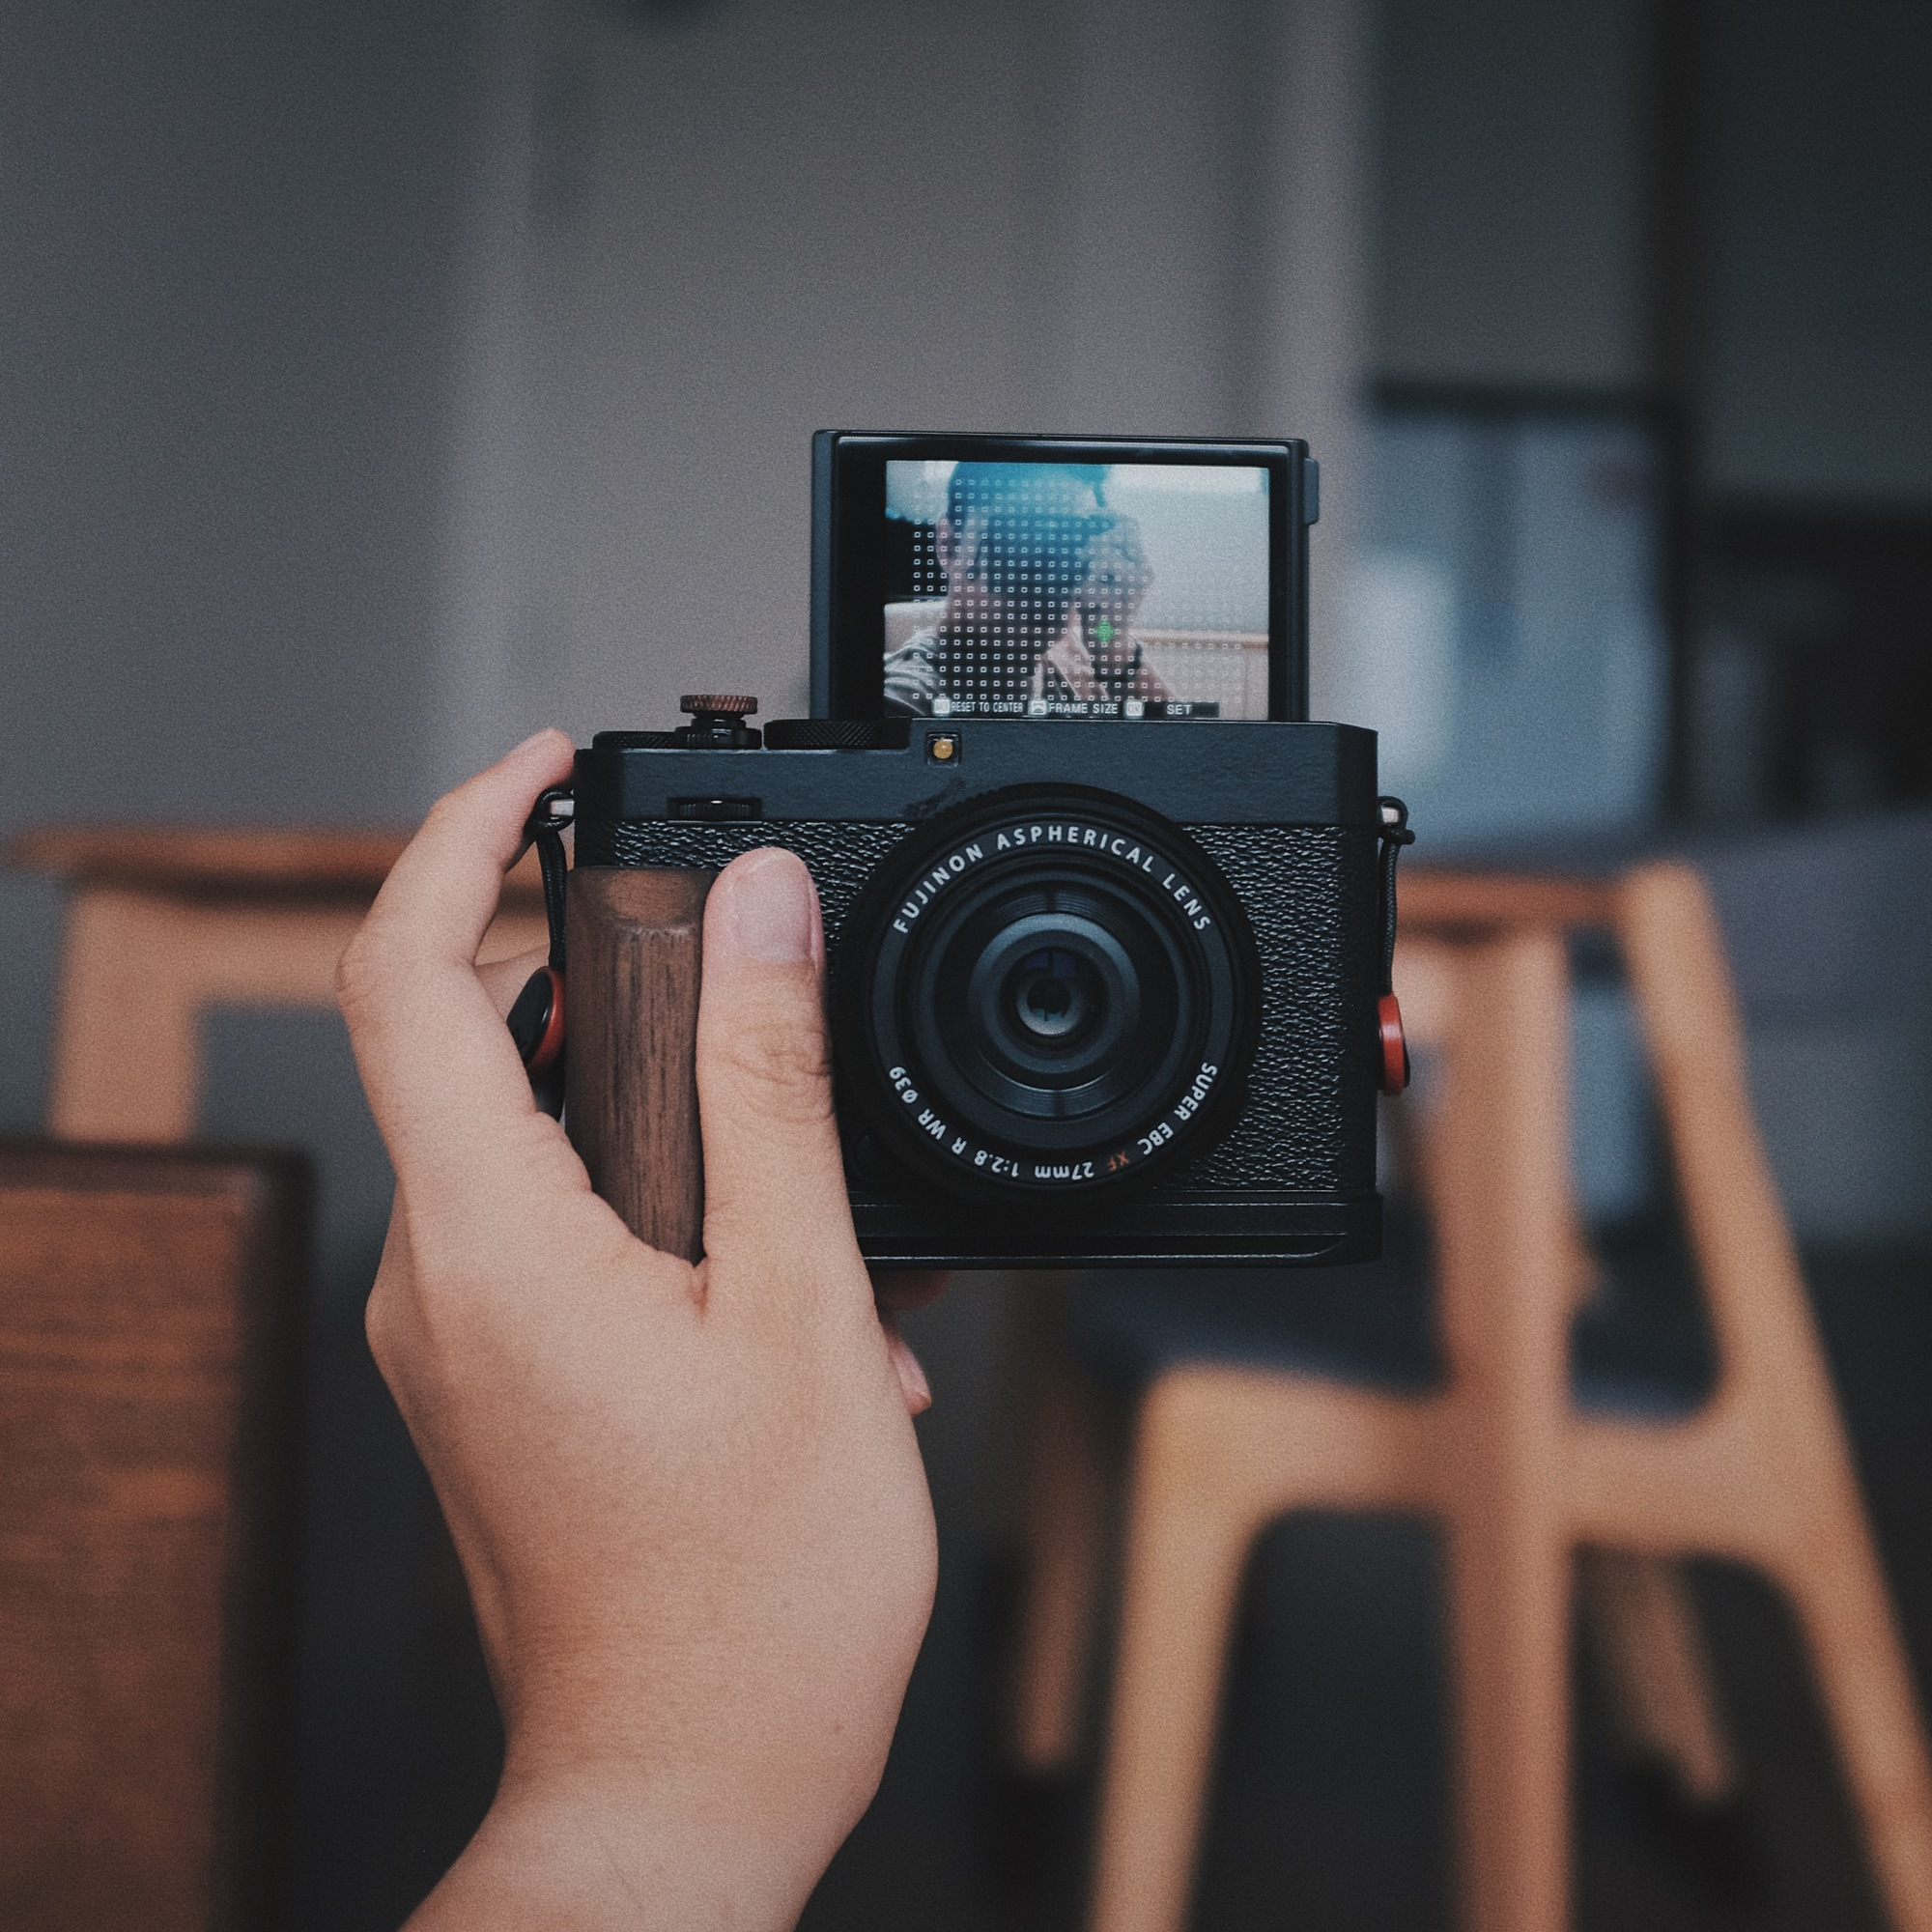
\includegraphics[width=\linewidth]{\envfinaldir/coverpic-prod.jpg}\par
            % \vskip 30pt
            \vfill

            \normalsize\rmfamily\scshape
            \copyright{} The Web Digest Project \hfill\large \envdatestr
        \end{center}
    \end{titlepage}
    % \restoregeometry
}
\newcommand{\simplehref}[1]{%
    \textcolor{blue!80!green}{\href{#1}{#1}}%
}
\renewcommand{\contentsname}{\center\Huge\sffamily\bfseries Contents\par\vskip 20pt}
\newcounter{ipartcounter}
\setcounter{ipartcounter}{0}
\newcommand{\ipart}[1]{
    % \vskip 20pt
    \clearpage
    \stepcounter{ipartcounter}
    \phantomsection
    \addcontentsline{toc}{chapter}{#1}
    % \begin{center}
    %     \Huge
    %     \sffamily\bfseries
    %     #1
    % \end{center}
    % \vskip 20pt plus 7pt
}
\newcounter{ichaptercounter}
\setcounter{ichaptercounter}{0}
\newcommand{\ichapter}[1]{
    % \vskip 20pt
    \clearpage
    \stepcounter{ichaptercounter}
    \phantomsection
    \addcontentsline{toc}{section}{\numberline{\arabic{ichaptercounter}}#1}
    \begin{center}
        \Huge
        \sffamily\bfseries
        #1
    \end{center}
    \vskip 20pt plus 7pt
}
\newcommand{\entrytitlefont}[1]{\subsection*{\raggedright\Large\sffamily\bfseries#1}}
\newcommand{\entryitemGeneric}[2]{
    % argv: title, url
    \parbox{\linewidth}{
        \entrytitlefont{#1}\par\vskip 5pt
        \footnotesize\ttfamily\mdseries
        \simplehref{#2}
    }\vskip 11pt plus 11pt minus 1pt
}
\newcommand{\entryitemGithub}[3]{
    % argv: title, url, desc
    \parbox{\linewidth}{
        \entrytitlefont{#1}\par\vskip 5pt
        \footnotesize\ttfamily\mdseries
        \simplehref{#2}\par\vskip 5pt
        \small\rmfamily\mdseries#3
    }\vskip 11pt plus 11pt minus 1pt
}
\newcommand{\entryitemAp}[3]{
    % argv: title, url, desc
    \parbox{\linewidth}{
        \entrytitlefont{#1}\par\vskip 5pt
        \footnotesize\ttfamily\mdseries
        \simplehref{#2}\par\vskip 5pt
        \small\rmfamily\mdseries#3
    }\vskip 11pt plus 11pt minus 1pt
}
\newcommand{\entryitemHackernews}[3]{
    % argv: title, hnurl, rawurl
    % \parbox{\linewidth}{
    %     \entrytitlefont{#1}\par\vskip 5pt
    %     \footnotesize\ttfamily\mdseries
    %     \simplehref{#3}\par
    %     \textcolor{black!50}{\href{#2}{#2}}
    % }\vskip 11pt plus 11pt minus 1pt
    \begin{minipage}{\linewidth}
            \entrytitlefont{#1}\par\vskip 5pt
            \footnotesize\ttfamily\mdseries
            \simplehref{#3}\par
            \textcolor{black!50}{\href{#2}{#2}}
    \end{minipage}\par\vskip 11pt plus 11pt minus 1pt
}







\begin{document}

\makeheader

\tableofcontents\clearpage




\ipart{Developers}
\ichapter{Hacker News}
\entryitemTwoLinks{OpenAI o3 and o4-mini}{https://news.ycombinator.com/item?id=43707719}{https://openai.com/index/introducing-o3-and-o4-mini/}

\entryitemTwoLinks{Attention K-Mart Shoppers}{https://news.ycombinator.com/item?id=43706706}{https://archive.org/details/attentionkmartshoppers}

\entryitemTwoLinks{Darwin's children drew all over the "On the Origin of Species" manuscript (2014)}{https://news.ycombinator.com/item?id=43706037}{https://theappendix.net/posts/2014/02/darwins-children-drew-vegetable-battles-on-the-origin-of-species}

\entryitemTwoLinks{Kermit: A typeface for kids}{https://news.ycombinator.com/item?id=43704904}{https://microsoft.design/articles/introducing-kermit-a-typeface-for-kids/}

\entryitemTwoLinks{Nintendo Bled Atari Games to Death}{https://news.ycombinator.com/item?id=43704596}{https://thereader.mitpress.mit.edu/how-nintendo-bled-atari-games-to-death/}

\entryitemTwoLinks{JetBrains IDEs Go AI: Coding Agent, Smarter Assistance, Free Tier}{https://news.ycombinator.com/item?id=43704579}{https://blog.jetbrains.com/blog/2025/04/16/jetbrains-ides-go-ai/}

\entryitemTwoLinks{CVE Foundation Launched to Secure the Future of the CVE Program}{https://news.ycombinator.com/item?id=43704430}{https://www.thecvefoundation.org/home}

\entryitemTwoLinks{European Union Vulnerability Database (EUVD)}{https://news.ycombinator.com/item?id=43703949}{https://euvd.enisa.europa.eu/}

\entryitemTwoLinks{Anonymous Release 10TB Leaked Data Exposing Kremlin Assets, Russian Businesses}{https://news.ycombinator.com/item?id=43703812}{https://trendsnewsline.com/2025/04/15/anonymous-leaks-10tb-of-data-on-russia-shocking-revelations/}

\entryitemTwoLinks{A Postmortem of a Startup}{https://news.ycombinator.com/item?id=43703682}{https://buildwithtract.com/}

\entryitemTwoLinks{An Introduction to Stochastic Calculus (2022)}{https://news.ycombinator.com/item?id=43703623}{https://bjlkeng.io/posts/an-introduction-to-stochastic-calculus/}

\entryitemTwoLinks{Markov Chain Monte Carlo Without All the Bullshit (2015)}{https://news.ycombinator.com/item?id=43700633}{https://www.jeremykun.com/2015/04/06/markov-chain-monte-carlo-without-all-the-bullshit/}

\entryitemTwoLinks{CVE program faces swift end after DHS fails to renew contract}{https://news.ycombinator.com/item?id=43700607}{https://www.csoonline.com/article/3963190/cve-program-faces-swift-end-after-dhs-fails-to-renew-contract-leaving-security-flaw-tracking-in-limbo.html}

\entryitemTwoLinks{Homeland Security funding for CVE program expires}{https://news.ycombinator.com/item?id=43700258}{https://www.theregister.com/2025/04/16/homeland\_security\_funding\_for\_cve/}

\entryitemTwoLinks{How dairy robots are changing work for cows and farmers}{https://news.ycombinator.com/item?id=43699188}{https://spectrum.ieee.org/lely-dairy-robots}

\entryitemTwoLinks{What the hell is a target triple?}{https://news.ycombinator.com/item?id=43696756}{https://mcyoung.xyz/2025/04/14/target-triples/}

\entryitemTwoLinks{The last RadioShack in Maryland is closing}{https://news.ycombinator.com/item?id=43696334}{https://marylandmatters.org/2025/04/14/end-of-an-era-the-last-radioshack-in-maryland-is-closing-its-doors/}

\entryitemTwoLinks{I speak at Harvard as it faces its biggest crisis since 1636}{https://news.ycombinator.com/item?id=43696010}{https://scottaaronson.blog/?p=8805}

\entryitemTwoLinks{The case of the UI thread that hung in a kernel call}{https://news.ycombinator.com/item?id=43695723}{https://devblogs.microsoft.com/oldnewthing/20250411-00/?p=111066}

\entryitemTwoLinks{It's easier than ever to de-censor videos}{https://news.ycombinator.com/item?id=43695701}{https://www.jeffgeerling.com/blog/2025/its-easier-ever-de-censor-videos}\ichapter{Phoronix}
\entryitemGeneric{\hskip 0pt{}Fedora 43 Looking To Make It Easier To Deploy Intel TDX Confidential VMs}{https://www.phoronix.com/news/Fedora-43-Better-Intel-TDX}

\entryitemGeneric{\hskip 0pt{}Mesa's Old OpenCL "Clover" Driver Removed For Mesa 25.2}{https://www.phoronix.com/news/Mesa-25.2-Drops-Clover}

\entryitemGeneric{\hskip 0pt{}Intel's Newest Linux Driver Being Worked On For The Kernel: iXD}{https://www.phoronix.com/news/Intel-Linux-iXD-Driver-Patches}

\entryitemGeneric{\hskip 0pt{}Mesa 25.1-rc1 Released With AMD RDNA4 Improvements, Lots Of RADV \& Intel ANV Additions}{https://www.phoronix.com/news/Mesa-25.1-rc1-Released}

\entryitemGeneric{\hskip 0pt{}NVIDIA 575.51.02 Linux Driver Beta Released With Smooth Motion Support}{https://www.phoronix.com/news/NVIDIA-575.51.02-Linux-Driver}

\entryitemGeneric{\hskip 0pt{}NVIDIA GeForce RTX 5060 Ti Linux GPU Compute Benchmarks}{https://www.phoronix.com/review/nvidia-rtx-5060-ti-linux-cuda}

\entryitemGeneric{\hskip 0pt{}Fedora 42 RISC-V Released - Builds For SiFive HiFive Premier P550 \& Milk-V Megrez}{https://www.phoronix.com/news/Fedora-42-RISC-V-Released}

\entryitemGeneric{\hskip 0pt{}FFmpeg's FFV1 Vulkan Decoder Now 3x Faster On AMD GPUs}{https://www.phoronix.com/news/FFmpeg-FFV1-Vulkan-AMD-3x}

\entryitemGeneric{\hskip 0pt{}More Radeon RX 9000 "RDNA4" Open-Source Driver Improvements Merged For Mesa 25.1}{https://www.phoronix.com/news/AMD-RDNA4-More-For-Mesa-25.1}\ichapter{Dribbble}
\entryitemGeneric{\hskip 0pt{}Startup Branding for Holidu: visual identity, brand design}{https://dribbble.com/shots/25903662-Startup-Branding-for-Holidu-visual-identity-brand-design}

\entryitemGeneric{\hskip 0pt{}Reindeer in Golden Light 🦌}{https://dribbble.com/shots/25905633-Reindeer-in-Golden-Light}

\entryitemGeneric{\hskip 0pt{}Logo Collection > Birds Volume 03}{https://dribbble.com/shots/25905911-Logo-Collection-Birds-Volume-03}

\entryitemGeneric{\hskip 0pt{}Altitude}{https://dribbble.com/shots/25902364-Altitude}

\entryitemGeneric{\hskip 0pt{}Automation builder - Wireframes}{https://dribbble.com/shots/25904187-Automation-builder-Wireframes}

\entryitemGeneric{\hskip 0pt{}Details - Amplemarket Logo \& Visual Identity}{https://dribbble.com/shots/25904732-Details-Amplemarket-Logo-Visual-Identity}

\entryitemGeneric{\hskip 0pt{}LogoLounge Book 15 Entry}{https://dribbble.com/shots/25904019-LogoLounge-Book-15-Entry}

\entryitemGeneric{\hskip 0pt{}Road Tripping}{https://dribbble.com/shots/25900418-Road-Tripping}

\entryitemGeneric{\hskip 0pt{}Lion sketches}{https://dribbble.com/shots/25898381-Lion-sketches}

\entryitemGeneric{\hskip 0pt{}Bloksy Logo Design - City, Colorful, Building, Construction}{https://dribbble.com/shots/25898764-Bloksy-Logo-Design-City-Colorful-Building-Construction}

\entryitemGeneric{\hskip 0pt{}Cute Shiba Catching a Ball}{https://dribbble.com/shots/25900210-Cute-Shiba-Catching-a-Ball}

\entryitemGeneric{\hskip 0pt{}Corti: Visual identity exploration}{https://dribbble.com/shots/25899331-Corti-Visual-identity-exploration}

\entryitemGeneric{\hskip 0pt{}Lume landing page interaction}{https://dribbble.com/shots/25898487-Lume-landing-page-interaction}

\entryitemGeneric{\hskip 0pt{}Watch}{https://dribbble.com/shots/25896863-Watch}

\entryitemGeneric{\hskip 0pt{}Chat App - Two Pages of Sketches}{https://dribbble.com/shots/25890352-Chat-App-Two-Pages-of-Sketches}

\entryitemGeneric{\hskip 0pt{}Nite Riot®\_Film Production // Case Study\_Vol.2.0}{https://dribbble.com/shots/25889874-Nite-Riot-Film-Production-Case-Study-Vol-2-0}

\entryitemGeneric{\hskip 0pt{}Simple vs Advanced}{https://dribbble.com/shots/25890403-Simple-vs-Advanced}

\entryitemGeneric{\hskip 0pt{}Lock Layer Logo Design - Shield, Letter L, Cube, Security}{https://dribbble.com/shots/25889313-Lock-Layer-Logo-Design-Shield-Letter-L-Cube-Security}

\entryitemGeneric{\hskip 0pt{}🔐 Cybersecurity Mobile App}{https://dribbble.com/shots/25887711--Cybersecurity-Mobile-App}

\entryitemGeneric{\hskip 0pt{}Lion}{https://dribbble.com/shots/25884438-Lion}

\entryitemGeneric{\hskip 0pt{}Hollo Logo Design}{https://dribbble.com/shots/25883411-Hollo-Logo-Design}

\entryitemGeneric{\hskip 0pt{}Adobe Acrobat Logo Redesign Concept}{https://dribbble.com/shots/25884888-Adobe-Acrobat-Logo-Redesign-Concept}

\entryitemGeneric{\hskip 0pt{}Corti: Visual identity exploration}{https://dribbble.com/shots/25871312-Corti-Visual-identity-exploration}

\entryitemGeneric{\hskip 0pt{}Revolve Logo Design}{https://dribbble.com/shots/25885583-Revolve-Logo-Design}


\ipart{Developers~~~~(zh-Hans)}
\ichapter{Solidot}
\entryitemGeneric{\hskip 0pt{}天文学家绘制星际冰地图}{https://www.solidot.org/story?sid=81069}

\entryitemGeneric{\hskip 0pt{}OpenAI 正在构建社交网络}{https://www.solidot.org/story?sid=81068}

\entryitemGeneric{\hskip 0pt{}日本监管机构要求 Google 停止垄断行为}{https://www.solidot.org/story?sid=81056}

\entryitemGeneric{\hskip 0pt{}美国六大科技巨头被指十年逃避了近 2780 亿美元的公司税}{https://www.solidot.org/story?sid=81055}

\entryitemGeneric{\hskip 0pt{}科学家绘制鸡基因调控的详细图谱}{https://www.solidot.org/story?sid=81054}

\entryitemGeneric{\hskip 0pt{}能随意塑形的流体电池}{https://www.solidot.org/story?sid=81053}

\entryitemGeneric{\hskip 0pt{}Temu 在美国撤下了 Google Shopping 广告}{https://www.solidot.org/story?sid=81052}

\entryitemGeneric{\hskip 0pt{}英特尔以 44.6 亿美元将 Altera 控股权出售给私募}{https://www.solidot.org/story?sid=81051}

\entryitemGeneric{\hskip 0pt{}特朗普政府对哈佛暂停 22 亿美元拨款}{https://www.solidot.org/story?sid=81050}

\entryitemGeneric{\hskip 0pt{}Pinta 3.0 释出}{https://www.solidot.org/story?sid=81049}

\entryitemGeneric{\hskip 0pt{}微软警告 Windows 11 用户不要删除神秘的空文件夹}{https://www.solidot.org/story?sid=81048}

\entryitemGeneric{\hskip 0pt{}中国民航局颁发首批飞行出租车运营合格证}{https://www.solidot.org/story?sid=81047}

\entryitemGeneric{\hskip 0pt{}英国高级警官呼吁禁止 16 岁以下儿童使用社交媒体}{https://www.solidot.org/story?sid=81046}

\entryitemGeneric{\hskip 0pt{}2022 年全球逾 300 万儿童死于抗生素耐药性感染}{https://www.solidot.org/story?sid=81045}

\entryitemGeneric{\hskip 0pt{}4 岁儿童就支持少数服从多数}{https://www.solidot.org/story?sid=81044}

\entryitemGeneric{\hskip 0pt{}傅利叶推出开源人形机器人 Fourier N1}{https://www.solidot.org/story?sid=81043}

\entryitemGeneric{\hskip 0pt{}日本人口连续 14 年减少}{https://www.solidot.org/story?sid=81042}

\entryitemGeneric{\hskip 0pt{}OpenAI API 可能要求客户验证身份 }{https://www.solidot.org/story?sid=81041}

\entryitemGeneric{\hskip 0pt{}AO3 进入了新时代}{https://www.solidot.org/story?sid=81040}

\entryitemGeneric{\hskip 0pt{}乌鸦会几何学}{https://www.solidot.org/story?sid=81039}\ichapter{V2EX}
\entryitemGeneric{\hskip 0pt{}[问与答] 关于大同事件不太明白的地方}{https://www.v2ex.com/t/1126025}

\entryitemGeneric{\hskip 0pt{}[职场话题] 面试了三次,凉凉, 27 岁就要终结开发梦吗?}{https://www.v2ex.com/t/1126024}

\entryitemGeneric{\hskip 0pt{}[macOS] 15.4.1 可以更了,旧贴: 「提醒大家一下 15.4」}{https://www.v2ex.com/t/1126023}

\entryitemGeneric{\hskip 0pt{}[Python] 啊? PyCharm 免费了?什么情况}{https://www.v2ex.com/t/1126022}

\entryitemGeneric{\hskip 0pt{}[Visual Studio Code] 你觉得 vscode 中最好用的插件是什么}{https://www.v2ex.com/t/1126021}

\entryitemGeneric{\hskip 0pt{}[Ubuntu] vmware17 安装 ubuntu22.04.5,最后一步报错}{https://www.v2ex.com/t/1126019}

\entryitemGeneric{\hskip 0pt{}[Android] 针对安卓手机最厉害的数据恢复软件或者 app 是哪个}{https://www.v2ex.com/t/1126018}

\entryitemGeneric{\hskip 0pt{}[JetBrains] jetbrains.com 域名被墙了?}{https://www.v2ex.com/t/1126016}

\entryitemGeneric{\hskip 0pt{}[JetBrains] Jetbrains AI 也顶不住开始出 free tier 了}{https://www.v2ex.com/t/1126015}

\entryitemGeneric{\hskip 0pt{}[问与答] 我目前发现没有一个 AI 能正确按照单精度转换 16 进制数 47 B8 05 01}{https://www.v2ex.com/t/1126014}

\entryitemGeneric{\hskip 0pt{}[GitHub] GitHub 访问 PR 时会出现 HTTP 500 错误}{https://www.v2ex.com/t/1126012}

\entryitemGeneric{\hskip 0pt{}[杭州] 相亲贴-帮表妹找对象}{https://www.v2ex.com/t/1126010}

\entryitemGeneric{\hskip 0pt{}[职场话题] 程序员深入了解保险行业一年多,带出的人生感悟}{https://www.v2ex.com/t/1126009}

\entryitemGeneric{\hskip 0pt{}[分享发现] 现在可以添加元宝好友直接进行聊天了!}{https://www.v2ex.com/t/1126008}

\entryitemGeneric{\hskip 0pt{}[数据库] 咨询一个 mysql 两个表更新同步到 es 的问题}{https://www.v2ex.com/t/1126007}

\entryitemGeneric{\hskip 0pt{}[宽带症候群] 苏州电信 IPV6 突然没了}{https://www.v2ex.com/t/1126006}

\entryitemGeneric{\hskip 0pt{}[Apple] 求推荐适合 Mac 的外置摄像头}{https://www.v2ex.com/t/1126005}

\entryitemGeneric{\hskip 0pt{}[分享创造] 最近有点上瘾的策略消除类游戏 blockblast unblocked 网页版}{https://www.v2ex.com/t/1126004}

\entryitemGeneric{\hskip 0pt{}[问与答] Lenny's Newsletter 兑换的 bolt 怎么兑换啊,一直提示出错}{https://www.v2ex.com/t/1126003}

\entryitemGeneric{\hskip 0pt{}[macOS] 老话题 MacOS 浏览器有什么推荐吗}{https://www.v2ex.com/t/1126002}

\entryitemGeneric{\hskip 0pt{}[问与答] 有哪位老哥知道这是哪个搜书的网站?}{https://www.v2ex.com/t/1126001}

\entryitemGeneric{\hskip 0pt{}[生活] [深夜小剧场]作为一个马上奔三成为魔法师的屌丝, 分享一下我对如今性别对立问题的思考}{https://www.v2ex.com/t/1126000}

\entryitemGeneric{\hskip 0pt{}[Visual Studio Code] 有用 VScode 远程开发的不服务器在美国延时 170~200 对开发影响大吗?}{https://www.v2ex.com/t/1125998}

\entryitemGeneric{\hskip 0pt{}[职场话题] 赴日 it 入职三个月,头也不回地准备辞职回国了}{https://www.v2ex.com/t/1125996}

\entryitemGeneric{\hskip 0pt{}[JetBrains] jetbrains 2025.1 发布了}{https://www.v2ex.com/t/1125994}

\entryitemGeneric{\hskip 0pt{}[Spotify] code 502}{https://www.v2ex.com/t/1125992}

\entryitemGeneric{\hskip 0pt{}[宽带症候群] 深圳联通 打击大上传流量宽带 告知函 最新版}{https://www.v2ex.com/t/1125991}

\entryitemGeneric{\hskip 0pt{}[青岛] 青岛的,出来冒个泡}{https://www.v2ex.com/t/1125990}

\entryitemGeneric{\hskip 0pt{}[程序员] react-aria-component/starter-kit 但是 vanilla-extract [anti utility-first css]}{https://www.v2ex.com/t/1125988}

\entryitemGeneric{\hskip 0pt{}[职场话题] 正式员工和公司签外包合同有啥坑吗}{https://www.v2ex.com/t/1125987}

\entryitemGeneric{\hskip 0pt{}[程序员] 请教,关于中后台 API 权限的设计方式?}{https://www.v2ex.com/t/1125986}

\entryitemGeneric{\hskip 0pt{}[操作系统] 请问,当我们在选择不同操作系统的时候,我们到底在选择什么?}{https://www.v2ex.com/t/1125983}

\entryitemGeneric{\hskip 0pt{}[JetBrains] 看起来 Toolbox App 支持远程开发了?}{https://www.v2ex.com/t/1125982}

\entryitemGeneric{\hskip 0pt{}[支付宝] 支付宝国际版首页加短视频了,你们有没有?}{https://www.v2ex.com/t/1125976}

\entryitemGeneric{\hskip 0pt{}[CSS] 技术文章翻译: CSS 实现极简的 LQIP}{https://www.v2ex.com/t/1125973}

\entryitemGeneric{\hskip 0pt{}[投资] 想到一个牛逼的股票交易策略,帮我看看靠谱不靠谱,能不能用 Python 实现}{https://www.v2ex.com/t/1125970}

\entryitemGeneric{\hskip 0pt{}[宽带症候群] 求一个异地回家/回国的组网方案}{https://www.v2ex.com/t/1125968}

\entryitemGeneric{\hskip 0pt{}[分享创造] 我写了一个帮助买房的 app}{https://www.v2ex.com/t/1125967}

\entryitemGeneric{\hskip 0pt{}[分享创造] 飞书 MCP function call 全场景 AI Agent}{https://www.v2ex.com/t/1125966}

\entryitemGeneric{\hskip 0pt{}[问与答] 想请教一下大家 ai 的一些应用场景}{https://www.v2ex.com/t/1125964}

\entryitemGeneric{\hskip 0pt{}[问与答] 动物 TTS}{https://www.v2ex.com/t/1125963}

\entryitemGeneric{\hskip 0pt{}[全球工单系统] 已经一个月了,通过搜索引擎搜索的微信文档,都是参数错误,难道是我被封禁了?大家正常吗}{https://www.v2ex.com/t/1125959}

\entryitemGeneric{\hskip 0pt{}[编程] 无需服务器部署官方 qq 机器人}{https://www.v2ex.com/t/1125958}

\entryitemGeneric{\hskip 0pt{}[问与答] 4 年前买的小米 AX6000 有没有换的必要?}{https://www.v2ex.com/t/1125956}

\entryitemGeneric{\hskip 0pt{}[Visual Studio Code] 第一次用 AI 写了一个 vscode 插件``Git Blame Annotations"}{https://www.v2ex.com/t/1125955}

\entryitemGeneric{\hskip 0pt{}[信息安全] 逆向工具 Rizin / radare2 (Cutter - Iaito) 时间线}{https://www.v2ex.com/t/1125954}

\entryitemGeneric{\hskip 0pt{}[Planet] @HomeZane}{https://www.v2ex.com/t/1125952}

\entryitemGeneric{\hskip 0pt{}[VXNA] 申请收录博客: datahonor.com/blog}{https://www.v2ex.com/t/1125951}

\entryitemGeneric{\hskip 0pt{}[远程工作] 做市交易系统架构师/Leader(远程办公/remote)}{https://www.v2ex.com/t/1125950}

\entryitemGeneric{\hskip 0pt{}[问与答] Vmware 虚拟机 win11 系统插入 iPhone 不识别怎么解决?}{https://www.v2ex.com/t/1125949}


\ipart{Generic News}







\clearpage
\leavevmode\vfill
\footnotesize

Copyright \copyright{} 2023-2025 Neruthes and other contributors.

This document is published with CC BY-NC-ND 4.0 license.

The entries listed in this newsletter may be copyrighted by their respective creators.

This newsletter is generated by the Web Digest project.

The newsletters are also delivered via Telegram channel \CJKunderline{\href{https://t.me/webdigestchannel}{https://t.me/webdigestchannel}}.\\
RSS feed is available at \CJKunderline{\href{https://webdigest.pages.dev/rss.xml}{https://webdigest.pages.dev/rss.xml}}.

This newsletter is available in PDF at
\CJKunderline{\href{https://webdigest.pages.dev/}{https://webdigest.pages.dev/}}.

The source code being used to generate this newsletter is available at\\
\CJKunderline{\href{https://github.com/neruthes/webdigest}{https://github.com/neruthes/webdigest}}.

This newsletter is also available in
\CJKunderline{\href{http://webdigest.pages.dev/readhtml/\envyear/WebDigest-20250417.html}{HTML}} and
\CJKunderline{\href{https://github.com/neruthes/webdigest/blob/master/markdown/\envyear/WebDigest-20250417.md}{Markdown}}.


\coverpic{https://unsplash.com/photos/a-small-bird-rests-on-a-shrub-rIhvJDqBO0w}{Doncoombez}


\end{document}
